\section{Performance}\label{sec:performance}

\subsection{Method}
\code{tools/measure.py} measures GhostVault's own costs against the simulated GitHub, which runs in
the same process; the results are in \code{report/data/measurements.json}. Times are therefore
GhostVault's work plus the simulator's, plus an optional delay added to every request; they are not
GitHub's. What GitHub adds is reported separately, as counts of requests. Write pacing, which on
GitHub spaces writes at least one second apart, is turned off for the timing, and its cost is given
instead as a lower bound: one second per write request. Each measurement runs twice, once for time and
requests and once, traced, for peak memory, because tracing slows Python down. Peak memory is what
Python allocates during the operation, minus the simulated GitHub's copy of the blobs. The machine was a
virtual machine with two cores of an Intel Xeon at 2.10\,GHz, Linux 6.18, Python 3.13.14 and
\code{cryptography} 50.0.1 with OpenSSL 4.0.2, using two repositories and the default distributed placement. The measurements and the stress runs were made on the code as it was just before the final validation check of \secref{sec:records} was added, one check per record read.

\subsection{Primitives}
Working on one 512\,KiB chunk at a time, AES-256-GCM encrypted at 1\,603\,MiB/s and decrypted at
1\,755\,MiB/s; SHA-256
ran at 1\,313\,MiB/s and the Git blob id at 1\,403\,MiB/s. Deriving a recovery bundle's key with the
default Argon2id parameters took 0.64\,s at best and 0.68\,s at the median of five runs. The
cryptography is far from being what limits GhostVault.

\subsection{Ghosting and restoring}
\tabref{tab:cycles} and \figref{fig:perf} show complete cycles of random (incompressible, non-image)
files of 1 to 256\,MiB. The requests a ghost makes follow from the design: one blob per chunk, then for
each repository one tree, one commit and one branch update, plus the reads that check the repository
and verify the upload; the first ghost in an empty repository also initialises it. A ghost of $n$
chunks over two repositories thus made $n+8$ writes here, $n+6$ in repositories already initialised.
A restore downloads each chunk once, reads the branches a few times, and makes six writes, the
deletion commits. Peak memory stayed between
3.5 and 6.5\,MiB whatever the file size, because chunks are streamed, and the data folder never held
more than the record: nothing is staged on disk.

\begin{table}[t]
\caption{Ghost and restore cycles (no added delay)}\label{tab:cycles}
\centering\footnotesize
\setlength{\tabcolsep}{4.2pt}
\begin{tabular}{@{}rrrrrrr@{}}
\toprule
& & \multicolumn{3}{c}{\textbf{Ghost}} & \multicolumn{2}{c}{\textbf{Restore}} \\
\cmidrule(lr){3-5}\cmidrule(l){6-7}
\textbf{MiB} & \textbf{Chunks} & \textbf{Time} & \textbf{Req.} & \textbf{Writes} & \textbf{Time} &
\textbf{Req.} \\
\midrule
1 & 2 & 0.037\,s & 24 & 10 & 0.041\,s & 22 \\
16 & 32 & 0.203\,s & 56 & 40 & 0.335\,s & 52 \\
64 & 128 & 0.875\,s & 152 & 136 & 1.263\,s & 148 \\
256 & 512 & 4.189\,s & 536 & 520 & 4.585\,s & 532 \\
\bottomrule
\end{tabular}

\vspace{2pt}\raggedright\scriptsize Two repositories, each initialised by the ghost. A restore always
made 6 writes. With 20\,ms added to every request: 1\,MiB, ghost 0.533\,s, restore 0.471\,s;
16\,MiB, ghost 1.406\,s, restore 0.730\,s.
\end{table}

\begin{figure}[t]
\centering
% Fig.: time of a ghost and of a restore against the simulated GitHub (report/data/measurements.json),
% and the lower bound GitHub's write pacing puts on the same operations.
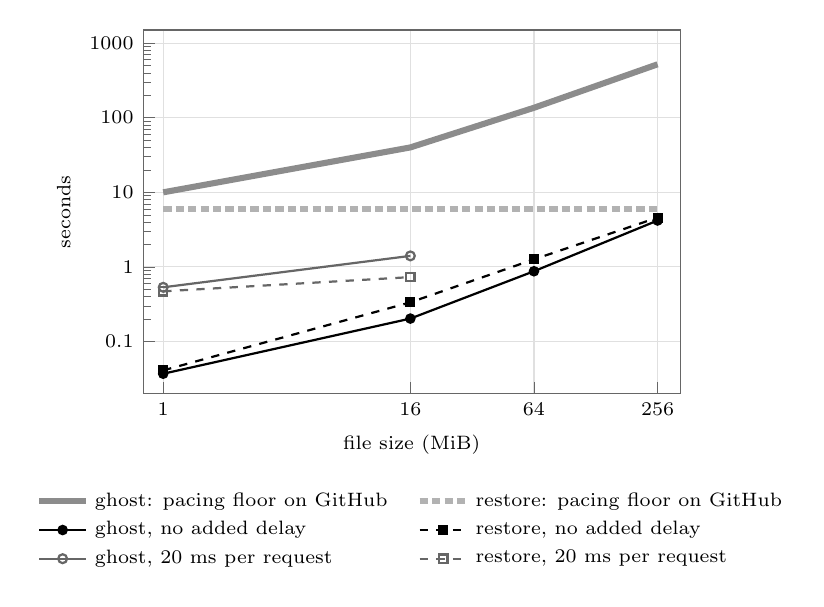
\begin{tikzpicture}
\begin{loglogaxis}[
  width=84mm, height=62mm,
  font=\scriptsize,
  xlabel={file size (MiB)}, ylabel={seconds},
  xmin=0.8, xmax=330, ymin=0.02, ymax=1500,
  xtick={1,16,64,256}, xticklabels={1,16,64,256},
  ytick={0.1,1,10,100,1000}, yticklabels={0.1,1,10,100,1000},
  grid=major, grid style={black!12},
  axis line style={black!60}, tick style={black!60},
  xtick pos=bottom, ytick pos=left,
  legend columns=2,
  legend style={font=\scriptsize, draw=none, at={(0.5,-0.24)}, anchor=north, cells={anchor=west},
                /tikz/every even column/.append style={column sep=3mm}},
  legend cell align=left,
  every axis plot/.append style={every mark/.append style={solid}},
]
\addplot[black!45, line width=2.2pt, mark=none] coordinates {(1,10) (16,40) (64,136) (256,520)};
\addlegendentry{ghost: pacing floor on GitHub}
\addplot[black!30, line width=2.2pt, mark=none, dash pattern=on 3pt off 1.5pt] coordinates {(1,6) (16,6) (64,6) (256,6)};
\addlegendentry{restore: pacing floor on GitHub}
\addplot[black, thick, mark=*, mark size=1.5pt] coordinates {(1,0.037) (16,0.203) (64,0.875) (256,4.189)};
\addlegendentry{ghost, no added delay}
\addplot[black, thick, mark=square*, mark size=1.4pt, dashed] coordinates {(1,0.041) (16,0.335) (64,1.263) (256,4.585)};
\addlegendentry{restore, no added delay}
\addplot[black!60, thick, mark=o, mark size=1.6pt] coordinates {(1,0.533) (16,1.406)};
\addlegendentry{ghost, 20 ms per request}
\addplot[black!60, thick, mark=square, mark size=1.5pt, dashed] coordinates {(1,0.471) (16,0.730)};
\addlegendentry{restore, 20 ms per request}
\end{loglogaxis}
\end{tikzpicture}

\caption{Time of a ghost and of a restore against the simulated GitHub, and the lower bound that
GitHub's write pacing (one write per second) puts on the same operations on GitHub. Both axes are
logarithmic. The 20\,ms series show the effect of request latency: a ghost's requests are sequential,
while a restore downloads eight chunks at a time.}
\label{fig:perf}
\end{figure}

\subsection{What GitHub adds}
On GitHub the floor dominates. At one write per second, a ghost of 256\,MiB needs at least 520\,s,
whatever the network: GhostVault can upload at most 512\,KiB per second, about 1.76\,GiB per hour,
before transfer time is even counted, and each chunk travels as base64 inside JSON, a third larger
than its ciphertext. GitHub also limits content creation to 80 requests per minute and 500 per
hour~\cite{gh-rate}, without listing which endpoints count. If blob creation counts against the hourly
limit, an account can store at most about 250\,MiB of chunks per hour, and GhostVault waits whenever
GitHub signals the limit. None of these costs was measured on GitHub. A restore is bound instead by
download bandwidth and by the primary limit of 5\,000 requests per hour per token~\cite{gh-rate},
which corresponds to about 2.4\,GiB of chunks per hour. Removing a ghost costs a few writes per
repository, whatever its size.

\subsection{Many ghosts}
\tabref{tab:scaling} shows the costs that grow with the number of ghosts. Each record takes about
1.6\,KB. Listing and start-up recovery read and validate every record, which is linear and cheap. Making
a ghost, however, also reads every record, to check that its name is unique, so the cost per ghost
grows linearly with their number, from 0.026\,s with 100 ghosts to 0.124\,s with 3\,000; on GitHub,
where even a one-chunk ghost takes a few seconds of paced writes, this is still small.

\begin{table}[t]
\caption{Costs that grow with the number of ghosts}\label{tab:scaling}
\centering\footnotesize
\begin{tabular}{@{}rrrr@{}}
\toprule
\textbf{Ghosts} & \textbf{Ghost one more} & \textbf{List all} & \textbf{Start-up recovery} \\
\midrule
100 & 0.026\,s & 0.005\,s & 0.011\,s \\
1\,000 & 0.056\,s & 0.070\,s & 0.164\,s \\
3\,000 & 0.124\,s & 0.170\,s & 0.644\,s \\
\bottomrule
\end{tabular}

\vspace{2pt}\raggedright\scriptsize Ghosts of 100 bytes, one chunk each, without previews; ``ghost one
more'' is the average over all ghosts made.
\end{table}
